%%%%%%%%%%%%%%%%%%%%%%%%%%%%%%%%%%%%%%%%%
% Masters Thesis 
% LaTeX Template
%
% This template is based on a template by:
% Steve Gunn (http://users.ecs.soton.ac.uk/srg/softwaretools/document/templates/)
% Sunil Patel (http://www.sunilpatel.co.uk/thesis-template/)
%
% Template license:
% CC BY-NC-SA 3.0 (http://creativecommons.org/licenses/by-nc-sa/3.0/)
%
%%%%%%%%%%%%%%%%%%%%%%%%%%%%%%%%%%%%%%%%%

%----------------------------------------------------------------------------------------
%	PACKAGES AND OTHER DOCUMENT CONFIGURATIONS
%----------------------------------------------------------------------------------------

\documentclass[
11pt, % The default document font size, options: 10pt, 11pt, 12pt
%oneside, % Two side (alternating margins) for binding by default, uncomment to switch to one side
english, % ngerman for German
onehalfspacing, % Single line spacing, alternatives: onehalfspacing or doublespacing
%draft, % Uncomment to enable draft mode (no pictures, no links, overfull hboxes indicated)
%nolistspacing, % If the document is onehalfspacing or doublespacing, uncomment this to set spacing in lists to single
liststotoc, % Uncomment to add the list of figures/tables/etc to the table of contents
%toctotoc, % Uncomment to add the main table of contents to the table of contents
%parskip, % Uncomment to add space between paragraphs
%nohyperref, % Uncomment to not load the hyperref package
headsepline, % Uncomment to get a line under the header
%chapterinoneline, % Uncomment to place the chapter title next to the number on one line
%consistentlayout, % Uncomment to change the layout of the declaration, abstract and acknowledgements pages to match the default layout
]{MastersDoctoralThesis} % The class file specifying the document structure

\usepackage[utf8]{inputenc} % Required for inputting international characters
\usepackage[T1]{fontenc} % Output font encoding for international characters

\usepackage{mathpazo} % Use the Palatino font by default
\usepackage{xcolor}

\usepackage{hyperref}
\usepackage{url}
\usepackage{dirtree}
\usepackage[font=small]{caption}
\captionsetup{justification=raggedright,singlelinecheck=false}
\usepackage{subcaption}
\usepackage{rotating}
\usepackage{float}

\usepackage[backend=bibtex,
					 style=numeric,
					 natbib=true,
					 sorting=none]{biblatex} % Use the bibtex backend with the authoryear citation style (which resembles APA)

\addbibresource{bibliography_er.bib} % The filename of the bibliography

\usepackage[autostyle=true]{csquotes} % Required to generate language-dependent quotes in the bibliography

% Word-splitting tolerance to avoid it
%\pretolerance=2000
%\tolerance=3000
\pretolerance=10000
\tolerance=2000 
\emergencystretch=10pt

%----------------------------------------------------------------------------------------
%	MARGIN SETTINGS
%----------------------------------------------------------------------------------------

\geometry{
	paper=a4paper, % Change to letterpaper for US letter
	inner=2.5cm, % Inner margin
	outer=3.8cm, % Outer margin
	bindingoffset=.5cm, % Binding offset
	top=1.5cm, % Top margin
	bottom=1.5cm, % Bottom margin
	%showframe, % Uncomment to show how the type block is set on the page
}

%----------------------------------------------------------------------------------------
%	THESIS INFORMATION
%----------------------------------------------------------------------------------------

\thesistitle{Man-made Structures Detection from Space} % Your thesis title, this is used in the title and abstract, print it elsewhere with \ttitle
\supervisor{Dr. Jordi \textsc{Vitrià}} % Your supervisor's name, this is used in the title page, print it elsewhere with \supname
\supervisoremail{ }
\examiner{} % Your examiner's name, this is not currently used anywhere in the template, print it elsewhere with \examname
\degree{} % Your degree name, this is used in the title page and abstract, print it elsewhere with \degreename
\author{Eduard \textsc{Ribas Fernández}} % Your name, this is used in the title page and abstract, print it elsewhere with \authorname
\authoremail{ }
\addresses{} % Your address, this is not currently used anywhere in the template, print it elsewhere with \addressname

\subject{Data Science} % Your subject area, this is not currently used anywhere in the template, print it elsewhere with \subjectname
\keywords{} % Keywords for your thesis, this is not currently used anywhere in the template, print it elsewhere with \keywordnames
\university{\href{http://www.ub.edu}{Universitat de Barcelona}} % Your university's name and URL, this is used in the title page and abstract, print it elsewhere with \univname
\department{\href{http://department.university.com}{}} % Your department's name and URL, this is used in the title page and abstract, print it elsewhere with \deptname
\group{\href{http://researchgroup.university.com}{}} % Your research group's name and URL, this is used in the title page, print it elsewhere with \groupname
\faculty{\href{http://mat.ub.edu}{Facultat de Matemàtiques i Informàtica}} % Your faculty's name and URL, this is used in the title page and abstract, print it elsewhere with \facname

\AtBeginDocument{
\hypersetup{pdftitle=\ttitle} % Set the PDF's title to your title
\hypersetup{pdfauthor=\authorname} % Set the PDF's author to your name
\hypersetup{pdfkeywords=\keywordnames} % Set the PDF's keywords to your keywords
}

\begin{document}

\frontmatter % Use roman page numbering style (i, ii, iii, iv...) for the pre-content pages

\pagestyle{plain} % Default to the plain heading style until the thesis style is called for the body content

%----------------------------------------------------------------------------------------
%	TITLE PAGE
%----------------------------------------------------------------------------------------

\begin{titlepage}
\begin{center}

\vspace*{.06\textheight}
{\scshape\LARGE \univname\par}\vspace{1.5cm} % University name
\textsc{\Large Fundamentals of Data Science Master's Thesis}\\[0.5cm] % Thesis type

\HRule \\[0.4cm] % Horizontal line
{\huge \bfseries \ttitle\par}\vspace{0.4cm} % Thesis title
\HRule \\[1.5cm] % Horizontal line
 
\begin{minipage}[t]{0.4\textwidth}
\begin{flushleft} \large
\emph{Author:}\\
\href{mailto:\authemail}{\authorname} % Author name - remove the \href bracket to remove the link
\end{flushleft}
\end{minipage}
\begin{minipage}[t]{0.4\textwidth}
\begin{flushright} \large
\emph{Supervisor:} \\
\href{mailto:\supemail}{\supname} % Supervisor name - remove the \href bracket to remove the link  
\end{flushright}
\end{minipage}\\[3cm]
 
\vfill

\large \textit{A thesis submitted in partial fulfillment of the requirements\\ for the degree of MSc in Fundamentals of Data Science}\\[0.3cm] % University requirement text
\textit{in the}\\[0.4cm]
\facname\\[2cm] % Research group name and department name
 
\vfill

{\large \today}\\[4cm] % Date
%\graphics{Logo} % University/department logo - uncomment to place it
 
\vfill
\end{center}
\end{titlepage}

\include{Chapters/Commands}

%----------------------------------------------------------------------------------------
%	ABSTRACT PAGE
%----------------------------------------------------------------------------------------

\begin{abstract}
\addchaptertocentry{\abstractname} % Add the abstract to the table of contents
With the development of affordable and recurrent remote sensing technology, we can now access frequent geospatial information in different levels of detail, ranging from 100m to 0.01m. The task of detecting various types of man-made structure and man-induced change has become a key problem in remote sensing image analysis. 

In this work we focus on providing an answer to the question:
\begin{itemize}
	\item[] \textit{What is the optimal trade-off between resolution and cost when aiming at determining the existence of man-made structures in remote sensing images?}
\end{itemize}
Obtaining this value is important not only for designing optimal satellite sensors but also to use optimal data sources when developing data-based remote sensing products. At a global level, this knowledge contributes to understand the impact of our species on the planet.

Our approach is based on developing a Deep Learning detector to classify human impact on aerial images. In particular, we exploit recent advances of Convolutional Neural Networks (CNN) that were successfully used for object detection and scene classification. We apply transfer learning by integrating a ResNet pre-trained on ImageNet to perform image classification on datasets of few thousand aerial images that we have manually collected and annotated. Using this classification pipeline we are able to determine the existence of man-made structure with an accuracy of $95\%$ at the best resolution.

We study the performance of our detector for resolutions ranging from $0.3m$ to $16m$. We observe a linear decrease of the classification accuracy down to about $81\%$ at the lowest resolution. Furthermore, we estimate the cost associated to build, launch, capture, and process satellite images to detect human impact. We estimate that monitoring the entire land surface of the earth at $1m$ resolution amounts for about $\$15$ million. This cost increases by about two orders of magnitude at the best resolution studied here, and decreases by about one order of magnitude at a resolution of $10m$ per pixel. These results could be further improved by training a CNN on a labeled large scale remote sensing dataset. Nevertheless, our results suffice for studying the expansion of human kind using satellite imagery and provide valuable information for designing optimal satellite sensors.
\end{abstract}

%----------------------------------------------------------------------------------------
%	ACKNOWLEDGEMENTS
%----------------------------------------------------------------------------------------

\begin{acknowledgements}
\addchaptertocentry{\acknowledgementname} % Add the acknowledgements to the table of contents

First, \textbf{Peter Weber} and I would like to thank \textbf{Santi Seguí}, \textbf{Lluis Garrido}, and \textbf{Eloi Puertas} to serve as experts in our thesis committee.
We are very grateful to our thesis advisor \textbf{Jordi Vitrià} for close guidance and exceptionally constructive and creative ideas on how to afront the problems we encountered. His scientific instinct was indispensable in critical moments of the project.
We also want to thank \textbf{Marco Bressan} from Satellogic for fruitful discussions, support with material, and advice about tools and data sources. Further, we want to thank \textbf{Javier Marin} and \textbf{Aitor Lucas} (both from Satellogic) for the help with the datasets.

Finally, I would like to thank my colleague \textbf{Peter Weber} for the hard-work throughout all this project. His experience, perseverance and cooperation made possible to complete this thesis successfully.

\end{acknowledgements}



%----------------------------------------------------------------------------------------
%	THESIS CONTENT - CHAPTERS
%----------------------------------------------------------------------------------------

\mainmatter % Begin numeric (1,2,3...) page numbering

\pagestyle{thesis} % Return the page headers back to the "thesis" style

% Include the chapters of the thesis as separate files from the Chapters folder
% Uncomment the lines as you write the chapters

\tableofcontents

\include{Chapters/Chapter1_Introduction_er}

\chapter{The datasets} % Main chapter title

\label{Chapter2} % For referencing the chapter elsewhere, use \ref{Chapter1} 

%----------------------------------------------------------------------------------------

In this chapter we will give an overview of existing annotated aerial imagery datasets and outline the reasons why none of them is suitable for our investigation. Following this discussion, we will describe two approaches for obtaining our own labeled dataset.

\section{Requirements and considerations}

Before we go into the presentation of labeled datasets we discuss the requirements that the dataset needs to fulfill in order to serve for the investigation in this thesis project. As already introduced, we want to detect human impact on aerial images and determine the dependency on resolution per pixel of a chosen evaluation metric. Ideally, the range for the resolutions should scale from a few tens of centimeters to a few tens of meters, whereas the images with low resolution can be generated from the high resolution images by downsampling. With this in mind, we mainly need to consider three aspects for the dataset.

First, we need to have imagery data with labels that can be used to clearly distinguish between existing and non-existing human impact, respectively. This impact might be classified pixel wise, or as binary classification for the entire image, or as multi-class classification that can be translated into binary labeling. 

Second, we need a balanced dataset of approximately the same number of images for both classes, and a large variety of different terrains within each class. 

Finally, the images need to have a resolution per pixel which is equal or better than 1m. Also, the height and width of the images should measure at least $500\times500$ pixels, so that one has enough room for downsampling. 

\section{Existing datasets}

In table \ref{table:datasets} we summarize the most relevant remote sensing datasets with ground truth labels that can be found in literature. The datasets were collected using different publicly available data sources. These range from pure low-resolution satellite imagery (Sentinel-2) to high-resolution images taken with an aircraft (USGS\footnote{United States Geological Survey}) to a mix of different image sources (Google Earth). 

\begin{table}[h!]
	\begin{tabular}{l | l | l | l | l | l }
	name & source & images & resolution (m) & size (pixel) & categories \\
	\hline
	BigEarthNet \parencite{sumbul2019} & Sentinel-2 & 590,326 & 10, 20, 60 & 120, 60, 20 & $\sim$ 50 \\
	EuroSAT \parencite{helber2017}	& Sentinel-2 & 27,000  & 10 & 64  & 10 \\
	UCMerced \parencite{yang2010} & USGS & 2100 & 0.3 & 256 & 21 \\
	DeepSat \parencite{basu2015}  & USGS  & 405,000 & 1 & 28 & 6  \\
	AID \parencite{xia2016} & Google Earth & 10,000  & 0.5 - 8  & 600 & 30 \\
	PatternNet \parencite{zhou2017} & Google Earth & 30,400 & 0.06 - 4.69 & 256 & 38 \\
	\end{tabular}
	\captionsetup{width=1\linewidth}
	\caption{\textbf{Publicly available remote sensing datasets with labels.} The table  lists the name of the dataset together with the bibliographic reference. It also details the data source of the images. It contains a description about the number of images, the resolution of the images, the size of the square images in pixel, and the number of categories.}
	\label{table:datasets}	
\end{table}

The satellite images have a resolution of equal or larger than 10m and they are collected with the Sentinel-2 satellites of the European earth observation program Copernicus. Although the datasets from this source (BigEarthNet and EuroSat) are comparatively large, they do not suffice for our purpose, because the resolution is not good enough and the images are too small.

The USGS National Map Urban Area Imagery collection \parencite{usgs} was utilized to collect remote sensing datasets in the two works UCMerced and DeepSat, where the former is the dataset that comes closest to our requirements. It features an image resolution of 0.3m per pixel, and the images have a height and width of 256 pixels. However, out of the 21 categories only 2 belong to images without human impact, while the other 19 show man-made structures. The DeepSat dataset unfortunately consists of image patches which are only $28 \times 28$ large, so that we aren't able to study these images as function of resolution.

The datasets using Google Earth as data source are collected using either the Google Earth or the Google Maps application programming interface (API). These images vary in resolution as well as in their original data provider since Google accesses several data sources. Both datasets (AID and PatternNet) have about 30 categories with several hundred images in each category. Here, different categories have different pixel resolutions, and again most of the categories relate to urban areas so that we do not have sufficient images without human impact. Even the categories that in principle should not show human influence contain images that break this rule.

Overall, the main issue with these datasets stems from the fact that non of them was collected with the purpose to analyze the human footprint. Therefore they are very unbalanced, and do not contain sufficient variety of images for the classes without human influence. We hence decided to collect and label images by ourselves. In our first attempt we used the Google Maps API, but we finally decided to use datasets from the USGS aerial imagery collection.

\section{Google Maps datasource}

Google has a public API that allows for querying images from their service Google Maps \parencite{google_maps_api}. In its most basic form, the API accepts as input parameters a latitude (lat) and longitude (lon), a zoom, and the image size (in pixels). Given this set of parameters one can calculate the resolution in meter per pixel \parencite{gmaps_res_per_m}, which is given by
\begin{equation}
resolution \Big[\frac{meter}{pixel}\Big] = \frac{156543.03392 \cdot cos(\frac{lattitude \cdot \pi}{180})}{2 ^ {zoom}}.
\label{eq:gmaps_res_per_m}
\end{equation}

Then, we developed an automated pipeline to download several images from a given area, which was selected with different strategies, and for some desired resolutions. In our first approach, we selected images that were Gaussian distributed around a center location from a list of interesting latitude/longitude coordinates. Another way consisted in downloading randomly sampled locations from within a defined rectangle.

Although any of these approaches would have served to build a complete dataset in an automated fashion, we finally decided to use a different data source. According to advises from Satellogic, Google Maps images have one major drawback regarding the pixel resolution: the images there are an interpolation from different spectral bands, where the RGB color bands do not necessarily have the expected resolution. Therefore, the resolution estimated by Eq.~\ref{eq:gmaps_res_per_m} is not reliable for the three color channels. We did not further investigate into this issue and instead turned to a different solution, which is discussed next.

\section{USGS datasource}

\subsection{Getting the images}\label{usgs_data}

To be able to construct a balanced and representative dataset we were recommended to focus on images of the United States, because of the wealth of available high resolution aerial imagery data from USGS Earthexplorer \parencite{usgs}. A nice side effect of choosing the United States is that a large variety of images of different terrain and topology are available. We combined the aerial imagery datasets from USGS with additional information about land cover and land use from the USGS Land Cover Viewer \parencite{land_cover_viewer}, precisely to guarantee larger variety through the selection of data from distinct land use categories.

For the determination of relevant geographic locations we excluded cities and highly developed urban areas, and instead focused on unpopulated areas. Specifically, we limited our image search to the four land use categories \textbf{agriculture}, \textbf{shrubland-grassland}, \textbf{semi-desert}, and \textbf{forest-woodland} that can be found in the USGS Land Cover Viewer. Note that these categories served as a rough geographic orientation to pin down geolocations of interest, because not all the images could be assigned with absolute certainty to one unique category. 

Whenever possible, we also tried to collect images from both classes (man-made vs. natural) within a given area/terrain. Additionally, we selected many images from national parks because we found that it is significantly harder to find imagery data that does not show human influence.

Once an area was pointed out as a region of interest using the USGS Land Cove Viewer, we located it on USGS Earthexplorer and downloaded images from that area. In particular, we constructed two datasets with 0.3m and 1m resolution, respectively. The former was taken from the category High Resolution Orthoimagery and the latter from the category National Agriculture Imagery Program (NAIP). Note that the images in these categories usually have a height and a width of several thousand pixels, and hence occupy a few hundreds of Megabytes of disk space. We then cropped smaller images from the raw images, which will be discussed in more detail in the following section. Overall, we downloaded around 100 raw images for each dataset. An example of one of these images is shown in Figure \ref{fig:example-unproc}.

\begin{figure}[h!]
	\centering
	\captionsetup{width=1\linewidth}
	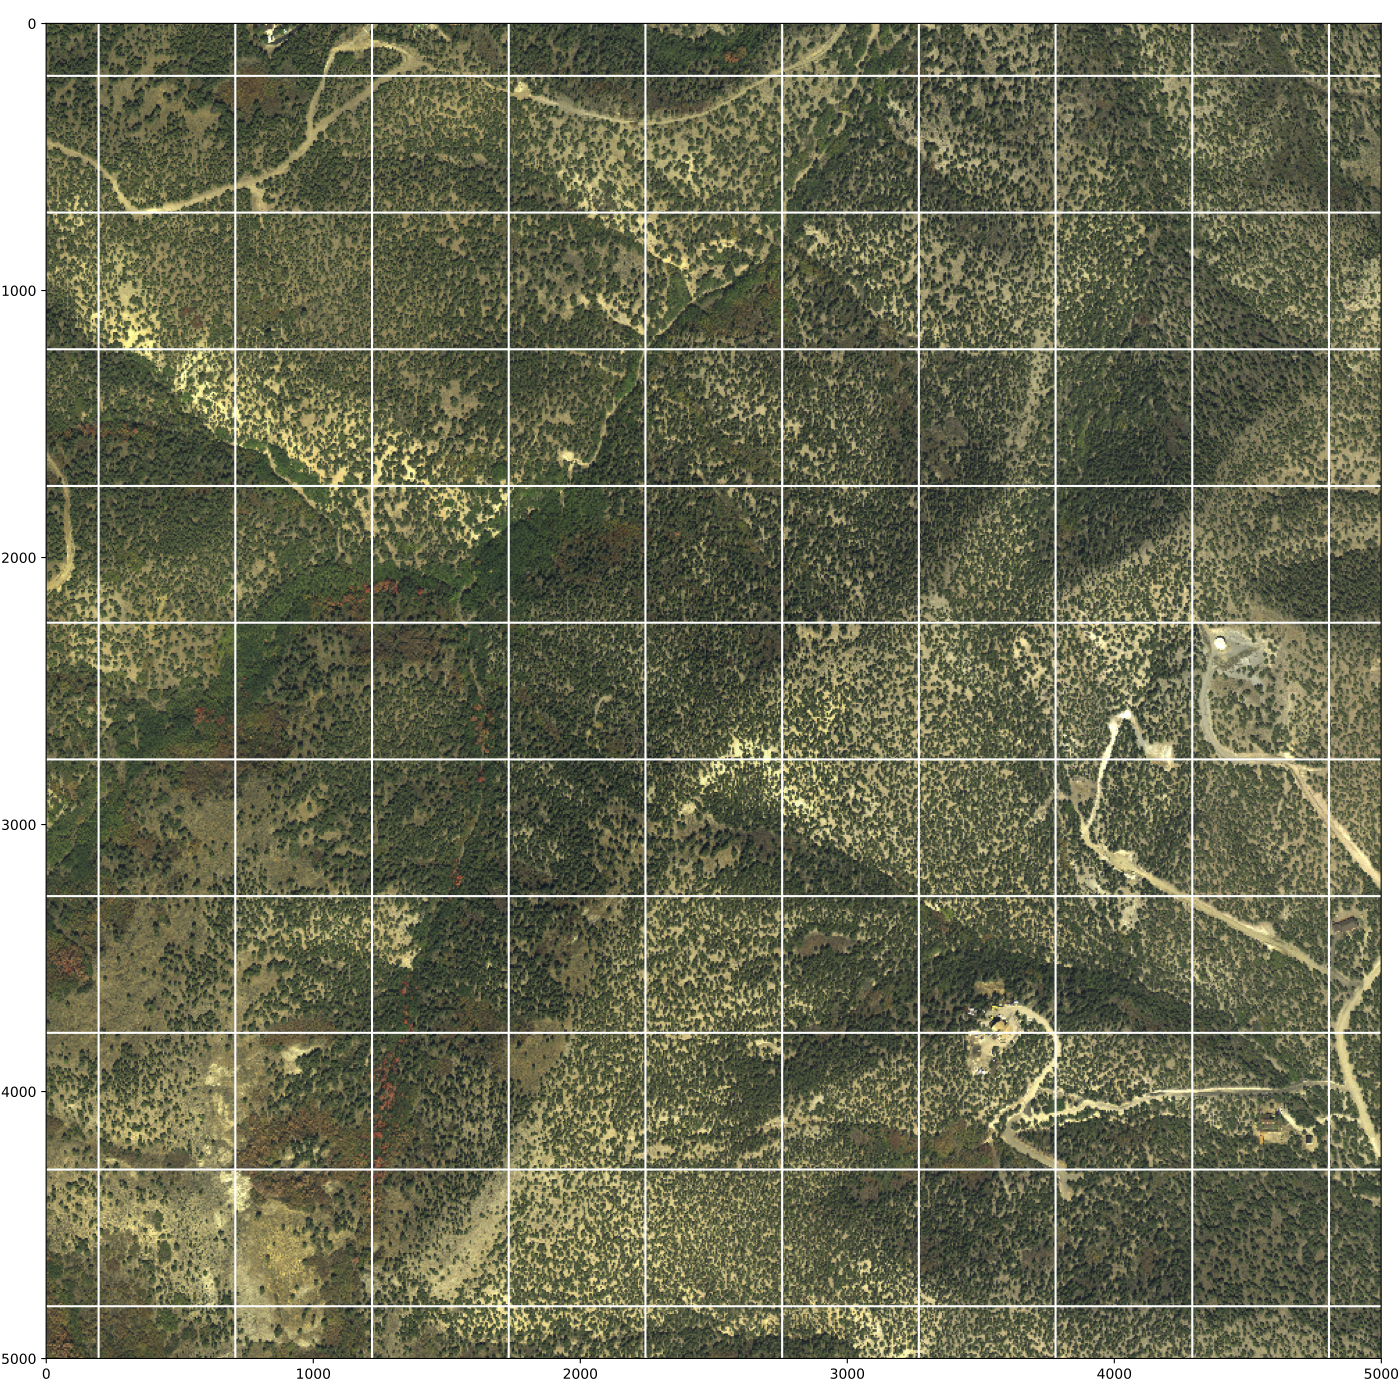
\includegraphics[width=0.95\textwidth]{Figures/example_unproc.pdf}
	\caption{\textbf{Example of unprocessed image.} This image has a size of $5000\times5000$ pixels. The continuous white lines show how we crop smaller images of size $512\times512$ pixels from the original one.}
	\label{fig:example-unproc}
\end{figure}

\subsection{Data processing and labeling}

Our data processing pipeline consists of the following steps:
\begin{enumerate}
	\item Download large raw images.
	\item Crop images of size $512\times512$ pixel.
	\item Label images with either zero (no human impact), one (minimal human impact), two (clear human impact).
	\item Degrade images i.e. reduce number of pixels and thereby resolution per pixel.
\end{enumerate}

Let us discuss each of these steps in more detail. An illustration of the first and second step of the image processing pipeline is given in Fig.~\ref{fig:example-unproc}. The white lines demonstrate the way we crop smaller images ($512\times512$ pixels) from the large raw image (in this case $5000\times5000$ pixels). We process all raw images in this manner, which yields approximately 80-150 processed images per raw image. We hence obtain about 10,000 processed images for each dataset. Then, within each category of the processed images we label a selected portion of the images by distributing the files into folders with the respective label name. 

We have published our datasets via a Google Drive link \parencite{datasets}. The image folder of the published datasets contains the raw images, the processed images, and the labeled images. In this folder we follow a specific folder structure, which is shown below. Here, pointy brackets (<parameter>) indicate a parameter and the content in the optional curly braces determines whether it is a folder pertaining to raw images. The first parameter is $pixels = 512$ and the second parameter represents the resolution of the dataset. Note that the label folders only exist in the case of processed images.
\vspace{10px}
\dirtree{%
	.1 \{raw-images-\}usgs-<pixels>-res<resolution>m.
	.2 semi-desert.
	.3 label-0.
	.3 label-1.
	.3 label-2.
	.2 agriculture.
	.3 label-2.
	.2 shrubland-grassland.
	.3 label-0.
	.3 label-1.
	.3 label-2.
	.2 semi-desert.
	.3 label-0.
	.3 label-1.
	.3 label-2.
}
\vspace{10px}

Annotating the images with labels was performed following certain rules, to ensure consistency and variety across the whole dataset.

First, we classified images with no human impact at all into the class with label zero, while we classified images with clear human influence into the class with label two. Ambiguous images i.e. images with minimal human traces, such as a small walking path, were classified into class one.

Also, we put major effort into creating datasets that contain images of similar texture spread across all classes. If we for example classified a set of images of a certain forest type into class zero we classified another set of images with a similar forest type, but containing a building or a street, into the class two. We followed the latter rule for all categories except for agriculture, as all images actually show human influence, and therefore classified all of them with label two. 

By sticking to these rules, we are able to guarantee that the algorithm learns features that relate to the appearance of man-made structures, and not to image artifacts such as color or texture.

\

Figures \ref{fig:agriculture_sample} - \ref{fig:desert-sample} display sample images for each of the four categories, repsectively. These images belong to the dataset that has a pixel resolution of 0.3m. The images from the 1m dataset have similar characteristics, but are not shown due to redundancy. Note that in Figs. \ref{fig:shrubland-sample} - \ref{fig:desert-sample} the first row represents images of label zero and the second row shows images that belong to label two. As mentioned above, the images in Fig.~\ref{fig:agriculture_sample} (agriculture) all contain human influence, and therefore belong to class two. 

\begin{figure}[H]
	\centering
	\captionsetup{width=1\linewidth}
	\includegraphics[width=1\textwidth]{Figures/agriculture_sample.pdf}
	\caption{\textbf{Example images of category Agriculture.} All images in this figure show clear signs of human impact. The images have a size of $512\times512$ pixels and a resolution of $0.3$m per pixel.}
	\label{fig:agriculture_sample}
\end{figure}

\begin{figure}[H]
	\centering
	\captionsetup{width=1\linewidth}
	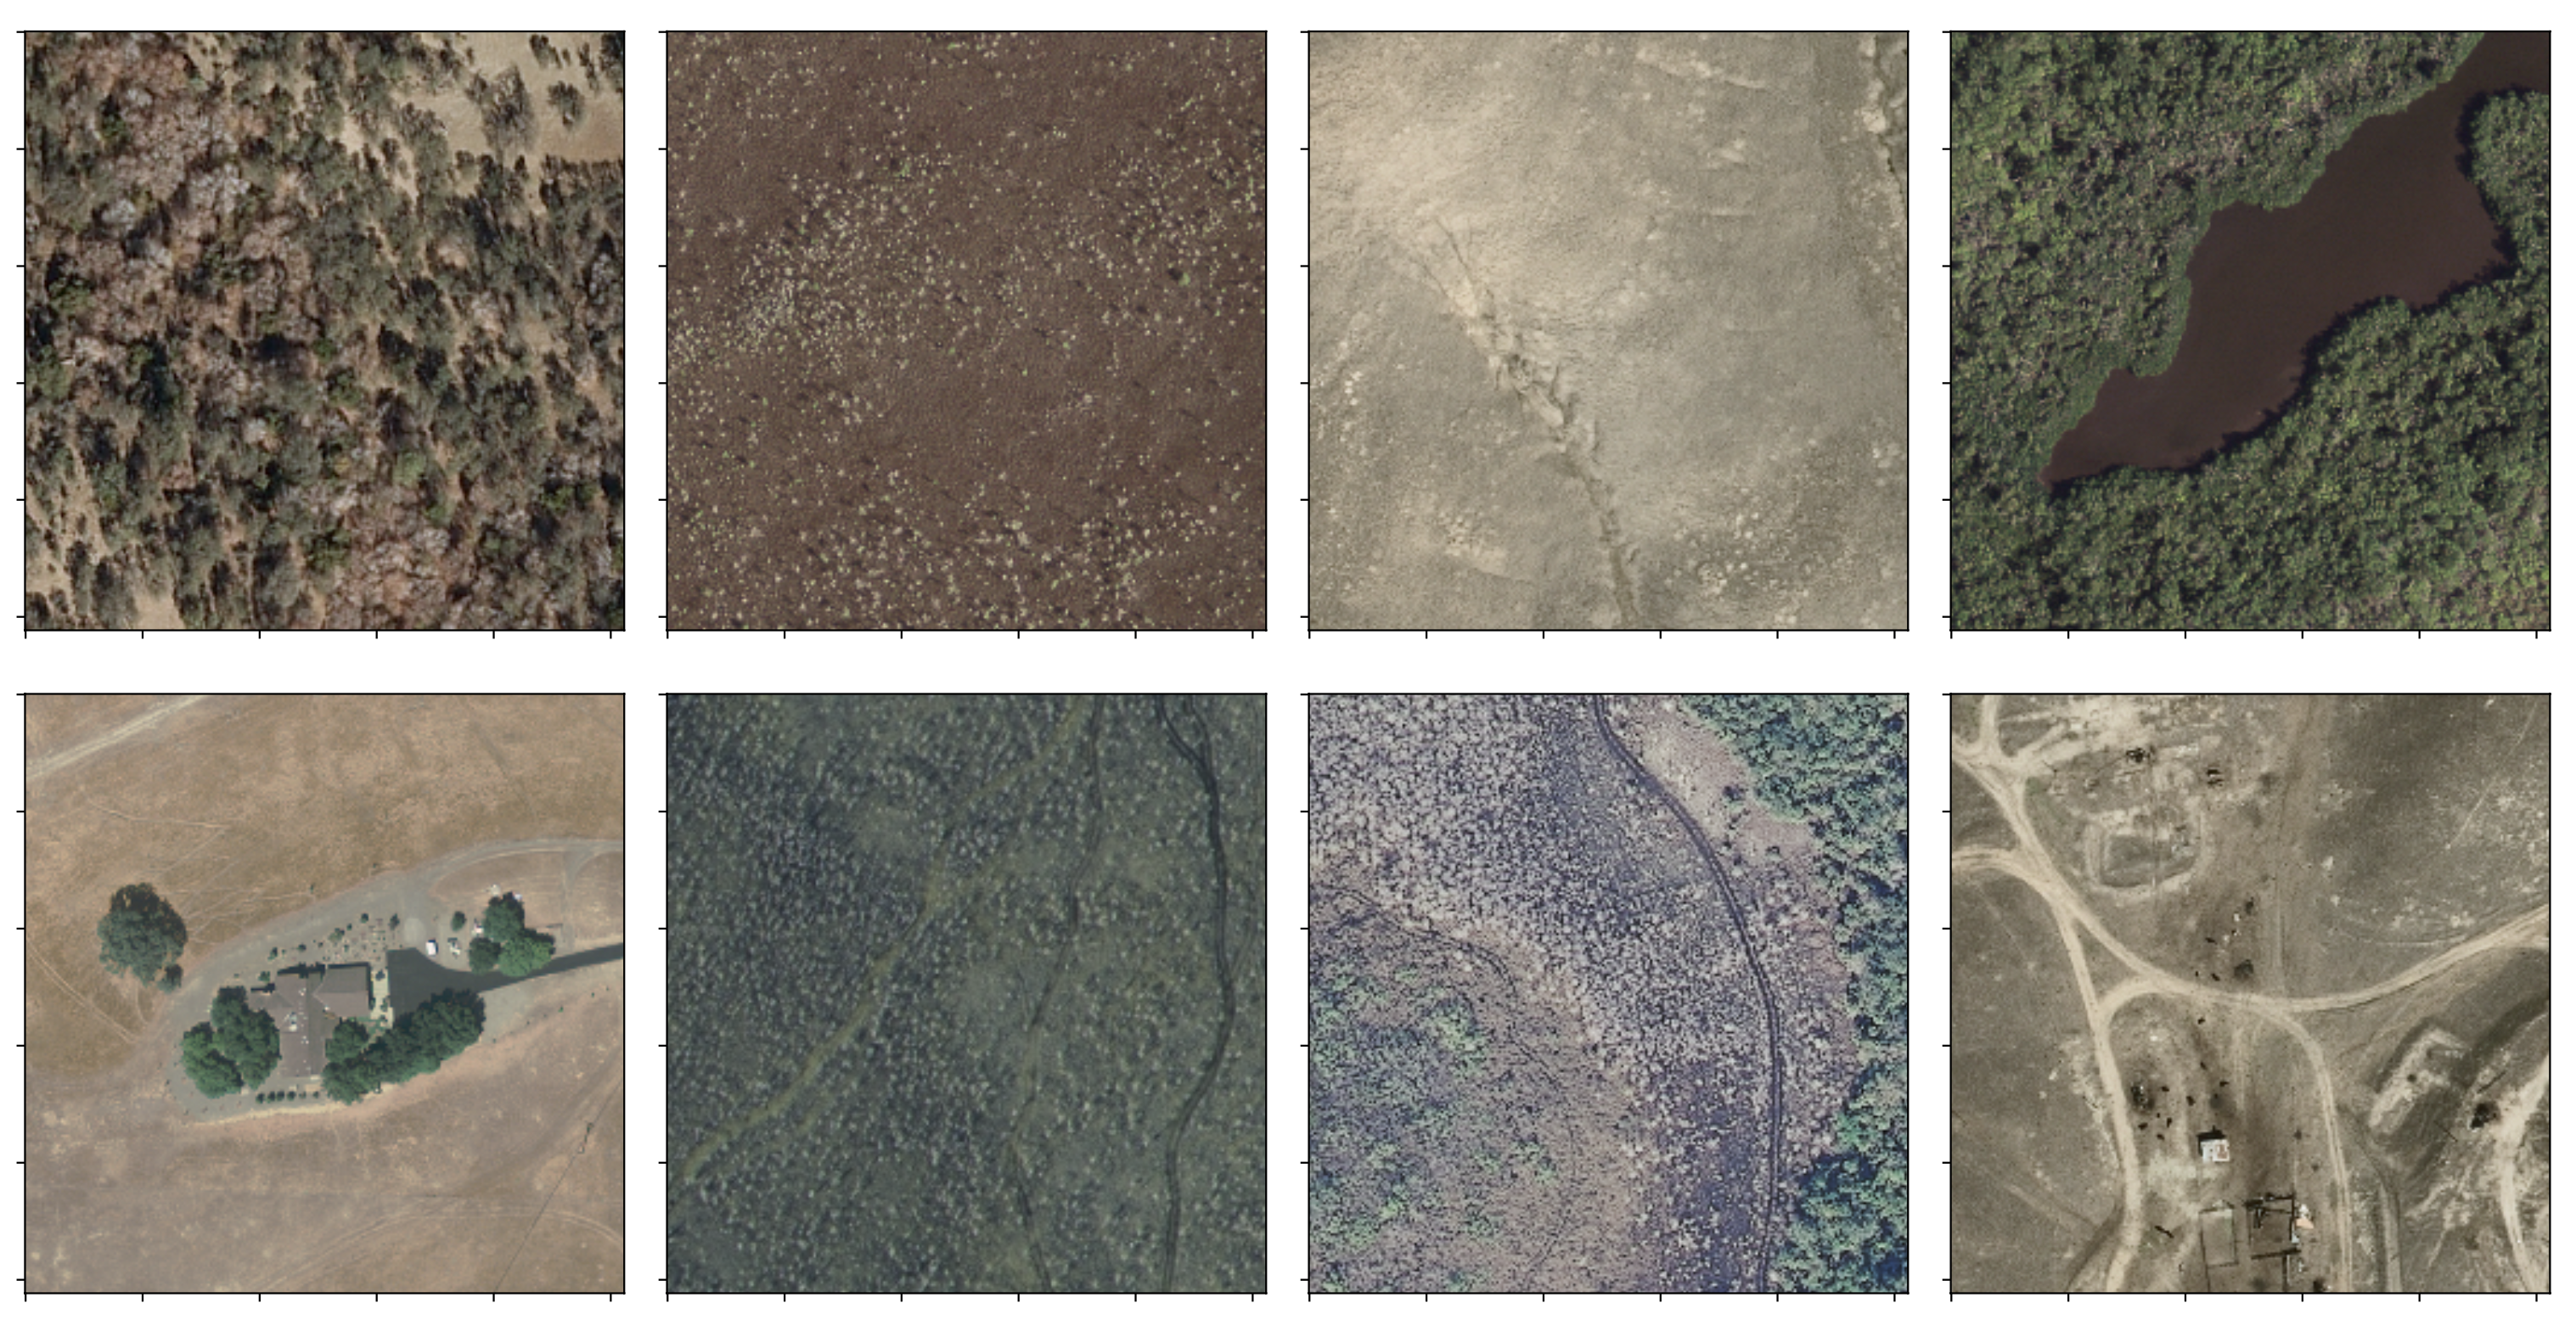
\includegraphics[width=1\textwidth]{Figures/shrubland-grassland_sample.pdf}
	\caption{\textbf{Example images of category shrubland-grassland.} The images in the first row do not contain any human influence, while the images in the second row show man-made structures. The images in this figure have a size of $512\times512$ pixels and a resolution of $0.3$m per pixel.}
	\label{fig:shrubland-sample}
\end{figure}

\begin{figure}[H]
	\centering
	\captionsetup{width=1\linewidth}
	\includegraphics[width=1\textwidth]{Figures/forest-woodland_sample.pdf}
	\caption{\textbf{Example images of category forest-woodland.} The images in the first row do not contain any human influence, while the images in the second row show man-made structures. The images in this figure have a size of $512\times512$ pixels and a resolution of $0.3$m per pixel.}
	\label{fig:forest-sample}
\end{figure}

\begin{figure}[H]
	\centering
	\captionsetup{width=1\linewidth}
	\includegraphics[width=1\textwidth]{Figures/semi-desert_sample.pdf}
	\caption{\textbf{Example images of category semi-desert.} The images in the first row do not contain any human influence, while the images in the second row show man-made structures. The images in this figure have a size of $512\times512$ pixels and a resolution of $0.3$m per pixel.}
	\label{fig:desert-sample}
\end{figure}

The distribution of categories and labels is shown in Fig.~\ref{fig:imstats}. Overall, for the 0.3m dataset we classified about 2200 images, and for the 1m dataset we classified about 1450 images. Our main goal consisted in creating a balanced dataset between label zero and label two as can be seen from the distributions. A minority of images, roughly $10\%$ of all annotated images were assigned to label one. These images were used at random to investigate the behaviour of the Machine Learning classifier, which is discussed in chapter~\ref{Chapter5}.

\begin{figure}[h!]
	\centering
	\captionsetup{width=1\linewidth}
	\includegraphics[width=1\textwidth]{Figures/imstats.pdf}
	\caption{\textbf{Number of images per category and label.} (a) Distribution of images for dataset with resolution of 0.3m per pixel. (b) Distribution of images for dataset with resolution of 1m per pixel.}
	\label{fig:imstats}
\end{figure}

\begin{figure}[h!]
	\centering
	\captionsetup{width=1\linewidth}
	\includegraphics[width=1\textwidth]{Figures/demo_degrade.pdf}
	\caption{\textbf{Example of image downsampling}. The upper left image has a base resolution of 0.3m per pixel and a size of $512\times512$ pixels whereas the lower right image has the worst resolution, 4.5m per pixel, and a size of $34\times34$ pixels. All intermediate images are downsampled by a factor corresponding to the resolution of the actual image divided by the base resolution. For instance, for the lower right image the factor is 15.}
	\label{fig:degrade}
\end{figure}

The last step of the data processing pipeline consisted in downsampling the processed and labeled images, in order to obtain images with a lower resolution. We used a Lanczos filter \parencite{duchon1979} for the sampling, which is based on a sinusoidal kernel. In Fig.~\ref{fig:degrade} we show a few selected resolutions for an example image from the agriculture category. Note that here we only schematically depict an example in order to illustrate the process. However, in our Machine Learning pipeline the images are downsampled on the fly and the result of this process is not stored on disk (see Section \ref{sec:dl_architecture} for further details).

For this particular image one can observe how certain image features disappear as the image quality is decreased. Above a resolution of around 3m per pixel one is not able anymore to identify the building close to the right corner of the image. 
The texture of the track that leads up to the building is blurred above a resolution of around 4m per pixel. This shows how different elements in an image are not recognizable anymore once the resolution approaches their characteristic size.



%----------------------------------------------------------------------------------------

\include{Chapters/Chapter3_NN_er} 
\include{Chapters/Chapter4_DLApproach_er} 
\include{Chapters/Chapter5_Results_er}

\chapter{Conclusions}

\label{Chapter6}

%----------------------------------------------------------------------------------------

In this final chapter we discuss and close the different aspects of the project, from the problem definition itself, to the datasets build and models developed, and we conclude our thesis with some further work ideas to continue and enhance our approach.

\section{The Problem}

The intial phase during the development of the project consisted on clearly defining the problem to study. The goal was to investigate which satellite imagery resolutions allowed for an accurate detection of man-made structures, and what would be the cost associated. For that, we needed to define the scope of human activity to consider, look for suitable datasets for this study (which eventually lead to building our own datasets), and define the actual technical problem to be modeled, in order to evaluate the accuracy by resolution. 

Both for the datasets and the problem, we needed them to be feasible enough to not require high technical and computational efforts (which would be, for instance, trying to detect every type of human activity in the images, providing their position and shape, and classifying them into several more categories). On the other hand, we needed it to be a realistic situation, so the results obtained could be extrapolated to other, more complex scenarios.

All in all, having a well-defined problem scope and a good approach to tackle it allowed us to achieve remarkable and realistic results.

\section{The Datasets}

After investigating existing datasets of labeled satellite images, we could not find the one suitable for our purpose, as most of them were mainly focused towards urban areas, or were just build for some other different goal that would not work for us. Hence, we decided to build it ourselves. It had to be representative enough to pose a challenge for our models, yet feasible to be build with our available time and resources. The four categories considered (agriculture, shrubland-grassland, semi-desert, and forest-woodland) and the balance between non-existent and existent human impact images allowed us to build a good and representative dataset, which makes reasonable to eventually generalize the results obtained to other scenarios.

Of course, we acknowledge that having a larger dataset of images, annotated with higher degree of detail, like position, shapes and types of man-made or natural structures, would be great to build high performance models, capable of detecting all sorts of human impact with far better accuracy. Nevertheless, this high-precision goal could not be fitted into our general purpose.

\section{The Models and Results}

Using a pre-trained CNN like the ResNet helped us to speed up the training process and achieve good results without requiring a very large dataset and computational power. The binary classification problem considered turned out to be feasible and representative of how accuracy is affected with a decrease in the image resolution. 

From the results we observe that, as expected, the higher the resolution the better, but also that there seems to be sweet spot between $1$-$2m$ and $8m$ where, except for the more subtle forms of human activity, most of the man-made structures studied are detectable with good accuracy. This trade-off with the resolution allows to consider more cost-economic satellite solutions without dramatically compromising accuracy and utility. For instance, operating a satellite at $2m$ (or $8m$) instead of $1m$ reduces the cost approximately by a factor 6 (or $100$).

\section{Future work}

With all that said, we realize that there is still plenty of space for further work and investigations, so let us now indicate some of these ideas.

First of all, having a better dataset could help improving the results and open new investigation lines to explore. It could be improved and enlarged with more variate images, with a better and more consistent classification, and including more detailed annotations of the position and type of objects or structures appearing. This would allow to train more accurate models capable of detecting all these kind of human impact.

Regarding the model, other techniques for feature extraction could be studied, like other pre-trained Neural Networks, and the parameters itself (like the number of activations to consider, the architecture of the model or the training phase) could be further fine-tuned. Additionally, the pipeline could be made more robust so that it could ingest a larger amount of data, as part of the improvements suggested for the dataset. And, of course, having a powerful computational cluster would allow to speed up the processes and target more ambitious goals.

A more in depth study of the results could help to understand more precisely on which images the algorithms fail, what kind of information are learning (patterns, colors, shapes, etc) and how to enhance them.

Finally, it would be interesting to have a more detailed analysis of the costs associated to all this solution, from data gathering, processing and modeling to the production implementation itself. Also, taking into account other related factors, like infrastructure needed, legal aspects and ecological footprint \parencite{Strubell2019} would give a more complete idea of the viability of global satellite image analysis.

\

In conclusion, this project has allowed us to investigate a relatively new topic, covering from the data gathering to the technical implementation using state-of-the-art tools, and leave the door open to further investigations.


%----------------------------------------------------------------------------------------
%	THESIS CONTENT - APPENDICES
%----------------------------------------------------------------------------------------

\appendix % Cue to tell LaTeX that the following "chapters" are Appendices

% Include the appendices of the thesis as separate files from the Appendices folder
% Uncomment the lines as you write the Appendices


\chapter{Tables} 

\label{Tables}

\begin{sidewaystable}
    \centering
	\begin{tabular}{rrrrrrrrrrrr}
\toprule
resolution (m) &  folds & \multicolumn{2}{c}{All categories} & \multicolumn{2}{c}{agriculture} & \multicolumn{2}{c}{forest-woodland} & \multicolumn{2}{c}{semi-desert} & \multicolumn{2}{c}{shrubland-grassland} \\
           &  &     mean acc. &    std &                 mean acc. &    std &                     mean acc. &    std &                 mean acc. &    std &                         mean acc. &    std \\
\midrule
       0.3 &     6 &   0.9226 & 0.0211 &               0.9850 & 0.0248 &                   0.8630 & 0.0624 &               0.8882 & 0.0453 &                       0.9561 & 0.0228 \\
       0.6 &     5 &   0.9383 & 0.0190 &               0.9699 & 0.0216 &                   0.8779 & 0.0269 &               0.9231 & 0.0410 &                       0.9748 & 0.0198 \\
       0.9 &     6 &   0.9347 & 0.0096 &               0.9439 & 0.0244 &                   0.8944 & 0.0561 &               0.9327 & 0.0216 &                       0.9578 & 0.0212 \\
       1.2 &     7 &   0.9271 & 0.0120 &               0.9488 & 0.0374 &                   0.9061 & 0.0373 &               0.9150 & 0.0328 &                       0.9399 & 0.0231 \\
       1.5 &     7 &   0.9288 & 0.0139 &               0.9622 & 0.0285 &                   0.8679 & 0.0383 &               0.9144 & 0.0309 &                       0.9604 & 0.0215 \\
       1.8 &     8 &   0.9224 & 0.0154 &               0.9678 & 0.0311 &                   0.8864 & 0.0650 &               0.9014 & 0.0363 &                       0.9371 & 0.0221 \\
       2.1 &     7 &   0.9108 & 0.0241 &               0.9618 & 0.0168 &                   0.8749 & 0.0454 &               0.8885 & 0.0571 &                       0.9216 & 0.0371 \\
       2.4 &     8 &   0.9120 & 0.0206 &               0.9573 & 0.0280 &                   0.8686 & 0.0590 &               0.8867 & 0.0358 &                       0.9352 & 0.0263 \\
       2.7 &     8 &   0.8952 & 0.0223 &               0.9620 & 0.0216 &                   0.8631 & 0.0191 &               0.8510 & 0.0350 &                       0.9117 & 0.0496 \\
       3.0 &     8 &   0.8893 & 0.0189 &               0.9571 & 0.0067 &                   0.8717 & 0.0197 &               0.8340 & 0.0472 &                       0.9055 & 0.0455 \\
       3.3 &     8 &   0.8957 & 0.0209 &               0.9539 & 0.0311 &                   0.8723 & 0.0479 &               0.8529 & 0.0341 &                       0.9121 & 0.0425 \\
       3.6 &     8 &   0.8784 & 0.0184 &               0.9415 & 0.0394 &                   0.8727 & 0.0442 &               0.8199 & 0.0348 &                       0.8935 & 0.0299 \\
       3.9 &     6 &   0.8819 & 0.0153 &               0.9456 & 0.0186 &                   0.8738 & 0.0330 &               0.8397 & 0.0364 &                       0.8796 & 0.0178 \\
       4.2 &     8 &   0.8804 & 0.0070 &               0.9389 & 0.0305 &                   0.8525 & 0.0267 &               0.8444 & 0.0533 &                       0.8961 & 0.0222 \\
       4.5 &     8 &   0.8715 & 0.0179 &               0.9383 & 0.0390 &                   0.8445 & 0.0308 &               0.8301 & 0.0340 &                       0.8821 & 0.0206 \\
       4.8 &     8 &   0.8690 & 0.0160 &               0.9508 & 0.0157 &                   0.8569 & 0.0517 &               0.7798 & 0.0456 &                       0.9035 & 0.0310 \\
\bottomrule
\end{tabular}

	\captionsetup{width=0.7\linewidth}
	\caption{\textbf{Aggregated cross-validation results for $0.3m$ dataset, $100$ neurons}}
	\label{tab:Results_03m_100n}
\end{sidewaystable}

\begin{sidewaystable}
    \centering
	\begin{tabular}{rrrrrrrrrrr}
\toprule
resolution (m) & \multicolumn{2}{c}{All categories} & \multicolumn{2}{c}{agriculture} & \multicolumn{2}{c}{forest-woodland} & \multicolumn{2}{c}{semi-desert} & \multicolumn{2}{c}{shrubland-grassland} \\
           &     mean acc. &    std &                 mean acc. &    std &                     mean acc. &    std &                 mean acc. &    std &                         mean acc. &    std \\
\midrule
       0.3 &   0.9335 & 0.0113 &               0.9540 & 0.0234 &                   0.8725 & 0.0946 &               0.9286 & 0.0253 &                       0.9613 & 0.0105 \\
       0.6 &   0.9565 & 0.0104 &               0.9663 & 0.0296 &                   0.9281 & 0.0304 &               0.9569 & 0.0120 &                       0.9671 & 0.0189 \\
       0.9 &   0.9406 & 0.0139 &               0.9515 & 0.0273 &                   0.9059 & 0.0264 &               0.9430 & 0.0314 &                       0.9550 & 0.0273 \\
       1.2 &   0.9390 & 0.0122 &               0.9559 & 0.0317 &                   0.8976 & 0.0483 &               0.9351 & 0.0336 &                       0.9622 & 0.0153 \\
       1.5 &   0.9249 & 0.0106 &               0.9696 & 0.0116 &                   0.8793 & 0.0443 &               0.8942 & 0.0250 &                       0.9536 & 0.0280 \\
       1.8 &   0.9198 & 0.0087 &               0.9627 & 0.0243 &                   0.8947 & 0.0439 &               0.8975 & 0.0404 &                       0.9312 & 0.0304 \\
       2.1 &   0.9065 & 0.0263 &               0.9638 & 0.0238 &                   0.8780 & 0.0597 &               0.8711 & 0.0541 &                       0.9190 & 0.0415 \\
       2.4 &   0.9209 & 0.0152 &               0.9689 & 0.0129 &                   0.8677 & 0.0247 &               0.9009 & 0.0354 &                       0.9435 & 0.0211 \\
       2.7 &   0.9021 & 0.0150 &               0.9644 & 0.0248 &                   0.8587 & 0.0327 &               0.8837 & 0.0426 &                       0.9111 & 0.0247 \\
       3.0 &   0.8957 & 0.0181 &               0.9568 & 0.0269 &                   0.8717 & 0.0440 &               0.8499 & 0.0597 &                       0.9112 & 0.0424 \\
       3.3 &   0.9086 & 0.0156 &               0.9679 & 0.0397 &                   0.8707 & 0.0345 &               0.8844 & 0.0426 &                       0.9183 & 0.0230 \\
       3.6 &   0.8878 & 0.0125 &               0.9669 & 0.0250 &                   0.8940 & 0.0402 &               0.8160 & 0.0339 &                       0.8940 & 0.0442 \\
       3.9 &   0.8804 & 0.0078 &               0.9495 & 0.0191 &                   0.8635 & 0.0345 &               0.8368 & 0.0365 &                       0.8853 & 0.0264 \\
       4.2 &   0.8774 & 0.0078 &               0.9405 & 0.0422 &                   0.8516 & 0.0330 &               0.8387 & 0.0374 &                       0.8923 & 0.0343 \\
       4.5 &   0.8745 & 0.0150 &               0.9428 & 0.0397 &                   0.8473 & 0.0493 &               0.8280 & 0.0328 &                       0.8886 & 0.0309 \\
       4.8 &   0.8774 & 0.0265 &               0.9505 & 0.0228 &                   0.8533 & 0.0404 &               0.8176 & 0.0497 &                       0.9000 & 0.0396 \\
\bottomrule
\end{tabular}

	\captionsetup{width=0.7\linewidth}
	\caption{\textbf{Aggregated cross-validation results for $0.3m$ dataset, $200$ neurons}}
	\label{tab:Results_03m_200n}
\end{sidewaystable}

\begin{sidewaystable}
    \centering
	\input{Tables/Results_1m_100n}
	\captionsetup{width=0.7\linewidth}
	\caption{\textbf{Aggregated cross-validation results for $1m$ dataset, $100$ neurons}}
	\label{tab:Results_1m_100n}
\end{sidewaystable}

\begin{sidewaystable}
    \centering
	\begin{tabular}{rrrrrrrrrrrr}
\toprule
resolution (m) &  folds & \multicolumn{2}{c}{All categories} & \multicolumn{2}{c}{agriculture} & \multicolumn{2}{c}{forest-woodland} & \multicolumn{2}{c}{semi-desert} & \multicolumn{2}{c}{shrubland-grassland} \\
           &  &     mean acc. &    std &                 mean acc. &    std &                     mean acc. &    std &                 mean acc. &    std &                         mean acc. &    std \\
\midrule
         1 &     5 &   0.8863 & 0.0305 &               0.9693 & 0.0432 &                   0.8661 & 0.0452 &               0.8974 & 0.0352 &                       0.8599 & 0.0377 \\
         2 &     5 &   0.8962 & 0.0156 &               0.9875 & 0.0280 &                   0.8951 & 0.0526 &               0.8819 & 0.0401 &                       0.8800 & 0.0472 \\
         3 &     5 &   0.8791 & 0.0267 &               0.9635 & 0.0519 &                   0.8713 & 0.0761 &               0.8873 & 0.0331 &                       0.8576 & 0.0336 \\
         4 &     8 &   0.8991 & 0.0339 &               0.9717 & 0.0317 &                   0.8999 & 0.0453 &               0.8734 & 0.0555 &                       0.9047 & 0.0529 \\
         5 &     5 &   0.8913 & 0.0301 &               0.9764 & 0.0324 &                   0.8823 & 0.0577 &               0.8591 & 0.0243 &                       0.9195 & 0.0495 \\
         6 &     8 &   0.8655 & 0.0194 &               0.9728 & 0.0450 &                   0.8609 & 0.0472 &               0.8341 & 0.0339 &                       0.8728 & 0.0542 \\
         7 &     6 &   0.8695 & 0.0321 &               0.9487 & 0.0588 &                   0.8789 & 0.0221 &               0.8327 & 0.0616 &                       0.8713 & 0.0669 \\
         8 &     7 &   0.8803 & 0.0230 &               0.9563 & 0.0592 &                   0.8702 & 0.0399 &               0.8625 & 0.0422 &                       0.8845 & 0.0144 \\
         9 &     7 &   0.8087 & 0.0378 &               0.9370 & 0.0706 &                   0.7727 & 0.0738 &               0.7832 & 0.0990 &                       0.8339 & 0.0819 \\
        10 &     7 &   0.8211 & 0.0352 &               0.9301 & 0.0634 &                   0.8172 & 0.0676 &               0.7900 & 0.0409 &                       0.8239 & 0.0698 \\
        11 &     8 &   0.8242 & 0.0130 &               0.9458 & 0.0604 &                   0.8250 & 0.0646 &               0.7849 & 0.0416 &                       0.8201 & 0.0414 \\
        12 &     8 &   0.8036 & 0.0252 &               0.9577 & 0.0473 &                   0.7817 & 0.0252 &               0.7695 & 0.0649 &                       0.8168 & 0.0588 \\
        13 &     8 &   0.8219 & 0.0408 &               0.9548 & 0.0384 &                   0.8040 & 0.0809 &               0.7870 & 0.0621 &                       0.8361 & 0.0494 \\
        14 &     6 &   0.8064 & 0.0343 &               0.9575 & 0.0374 &                   0.7846 & 0.0595 &               0.7743 & 0.0508 &                       0.8164 & 0.0592 \\
        15 &     8 &   0.7982 & 0.0368 &               0.9638 & 0.0397 &                   0.8004 & 0.0756 &               0.7330 & 0.0374 &                       0.8117 & 0.0625 \\
        16 &     8 &   0.7989 & 0.0247 &               0.9528 & 0.0466 &                   0.7636 & 0.0673 &               0.7708 & 0.0419 &                       0.8161 & 0.0446 \\
\bottomrule
\end{tabular}

	\captionsetup{width=0.7\linewidth}
	\caption{\textbf{Aggregated cross-validation results for $1m$ dataset, $200$ neurons}}
	\label{tab:Results_1m_200n}
\end{sidewaystable}


\chapter{Files and Code}

\label{FilesCode}

All the files used in this project, including the image datasets build and code generated, are available online:

\begin{itemize}

	\item The images datasets are published in Google Drive (see \href{https://drive.google.com/open?id=1Hjod1ZTuSIW3VNO2IuGoq_iagI3imnJQ}{link} or reference \parencite{datasets}).
	
	\item All the code produced and used in these analysis is available in a GitHub repository (see \href{https://github.com/peterweber85/MasterThesis}{link} or reference \parencite{github}). It includes Python libraries generated, scripts and Jupyter Notebooks.

\end{itemize}



\chapter{Author Contributions} % Main chapter title

\label{AuthorContributions}

This thesis is a group project between Eduard Ribas Fernández and Peter Weber. Here we will describe the individual contributions of each author. Overall, both authors have contributed to all parts in this project with different weights in each part.

In the first major block, the generation of the dataset, the distribution is as follows. The image search and download of the raw images was performed by P. Weber, while programming the image processing pipeline was done by both authors with similar weight. The labeling of the processed images was also done by both authors.

In the second major block, the data analysis pipeline, P. Weber has higher contribution at the beginning of the pipeline i.e. prototyping first solutions using transfer learning. E. Ribas has higher contribution towards the end of the pipeline. This includes optimizing the code for Colab, tuning the hyperparamters, performing analysis per category and producing the final figures.
Regarding estimation of the cost, both authors have equal contribution.

The same applies for preparing all documents related to this project (Github repository, high-level overview, thesis document), both authors have equally contributed.

%----------------------------------------------------------------------------------------
%	BIBLIOGRAPHY
%----------------------------------------------------------------------------------------

\printbibliography[heading=bibintoc]

%----------------------------------------------------------------------------------------

\end{document}  
